%!TEX TS-program = xelatex
%!TEX root = ../../maxwell2018thesis.tex

\chapter[Modelling SERP Level Stopping Behaviours]{Modelling~\gls{acr:serp} Level\\Stopping Behaviours}\label{chap:serp}
In Chapters~\ref{chap:snippets} and~\ref{chap:diversity}, we reported on two user studies that examined the effects of searcher behaviour and performance under different search contexts. Interaction data from these studies were then used to ground simulations of interaction that examined how each of the twelve different stopping strategies performed and approximated real-world searcher stopping behaviours. We now turn our attention towards providing a complete answer to our first high-level research question, \darkblueboxbold{HL-RQ1}.

\begin{itemize}
    \item{\darkblueboxbold{HL-RQ1} How can we improve searcher models to incorporate different stopping decision points?}
\end{itemize}

In order to address this research question, we presented in Chapter~\ref{chap:csm} the~\glsfirst{acr:csm}, a conceptual, high-level model of the search process. The~\gls{acr:csm} introduced the~\gls{acr:serp} level stopping decision point, motivated by information scent. This new stopping decision point allows a simulated searcher to \emph{abandon} a~\gls{acr:serp} if a general \emph{overview} of the given~\gls{acr:serp} shows that the results did not appear to provide promising results. With the definition of the~\gls{acr:csm} partially satisfying \darkblueboxbold{HL-RQ1}, in this we chapter provide the results of an empirical study using the new stopping decision point.

\section{Motivation and Research Questions}\label{sec:serp:background}
We begin with the concept of~\gls{acr:serp} abandonment (discussed previously in Section~\ref{sec:csm:assumptions:good_abandonment} on page~\pageref{sec:csm:assumptions:good_abandonment}), before considering how~\glsfirst{acr:ift} provides strong theoretical motivation. The concept behind the new~\gls{acr:serp} level stopping decision point revolves around the notion of~\gls{acr:serp} abandonment, when a searcher fails to click on any of the results returned for a given query~\citep{diriye2012abandonment, hassan2013serp_abandonment}. This may occur for a variety of reasons, both good and bad. The primary motivator for this study considers the notion of bad abandonment, where searchers abandon a~\gls{acr:serp} because they are dissatisfied by the results returned~\citep{hassan2013serp_abandonment}.

\begin{figure}[t!]
    \centering
    \resizebox{1\hsize}{!}{
    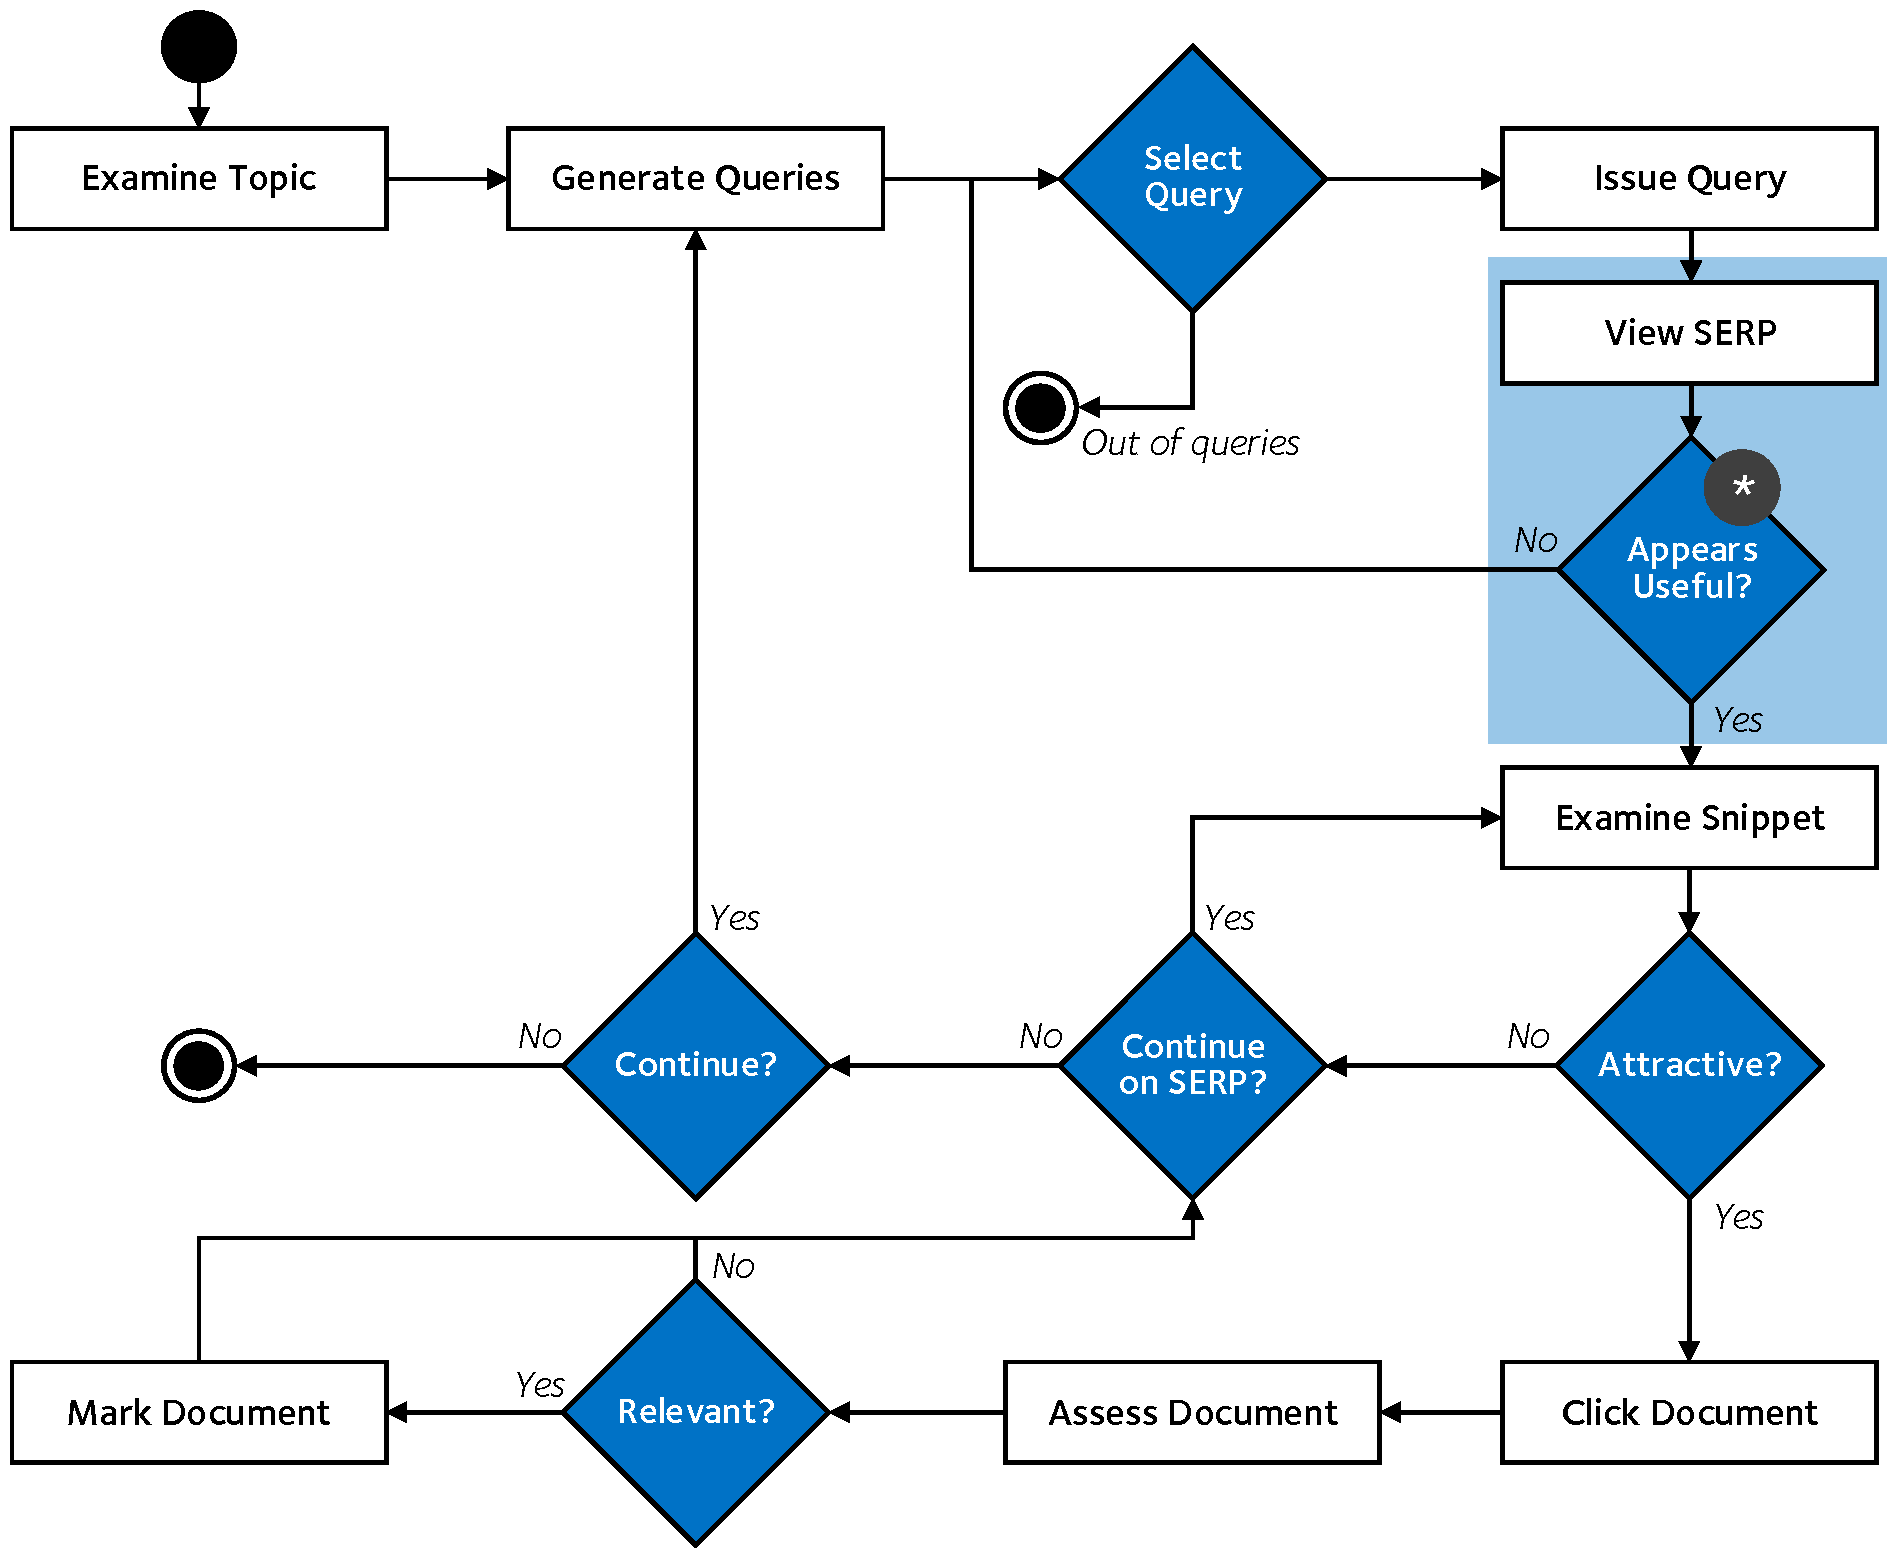
\includegraphics{figures/ch9-csm.pdf}}
    \caption[The~\gls{acr:csm} and~\gls{acr:serp} stopping point]{The~\glsfirst{acr:csm}, highlighting the stopping decision point (by an asterisk\emph{*}, with the~\gls{acr:serp} examination component also highlighted within the blue rectangle) that is examined in detail in this chapter. Refer to Section~\ref{sec:csm:flow} for an in-depth explanation of the model.}
    \label{fig:csm_ch9}
\end{figure}

%Motivated by \emph{information scent} and the \emph{patch model} -- both part of~\gls{acr:ift}\footnote{Refer to Section~\ref{sec:stopping_background:theoretical:ift} on page~\pageref{sec:stopping_background:theoretical:ift} for a detailed explanation of the patch model.} --

As we discussed in Section~\ref{sec:stopping_background:theoretical:ift:patch} on page~\pageref{sec:stopping_background:theoretical:ift:patch},~\cite{pirolli1999ift} argue that information seekers are like animals foraging in the wild, and as such will follow a scent to find food. As discussed previously, information seekers have been shown to follow a series of \emph{proximal cues} provided by~\gls{acr:serp} components such as hypertext links, titles, snippets and thumbnails to help locate relevant information~\citep{pirolli1995ift, pirolli1999ift, chi2001information_scent, oltston2003scenttrails, pirolli2007ift}. For example,~\cite{card2001scent_graphs} found that when navigating through webpages, searchers were more likely to leave when the information scent provided on a page began to decline. Work by~\cite{wu2014information_scent} discussed a user study where low, medium and high scent~\glsplural{acr:serp} were created by changing the number and distribution of relevant items on the page -- thus altering the proximal cues provided. Those interacting with high scent~\glsplural{acr:serp} examined more content and went to greater depths compared to those who utilised low scent~\glsplural{acr:serp}. Further work by~\cite{ong2017scent_behaviour} -- and indeed the user study reported in Section~\ref{chap:snippets:user} -- all confirm that modifying the scent of a~\gls{acr:serp} does indeed alter a searcher's stopping behaviour.

For this chapter, we operationalise the information scent as the performance of a given~\gls{acr:serp}, examining how the new~\gls{acr:serp} level stopping decision point within the searcher model -- as shown in Figure~\ref{fig:csm_ch9}\footnote{Further information on the~\glsfirst{acr:csm} can be found in Chapter~\ref{chap:csm}, starting on page~\pageref{chap:csm}.} -- affects searcher, stopping and overall performance. This is achieved by enumerating a series of different~\gls{acr:serp} level implementations, allowing us to operationalise the new stopping decision point in several ways. As such, we pose two key research questions to be addressed in this chapter.

\begin{itemize}
    \item[]{\darkblueboxbold{SERP-RQ1} Does the incorporation of a~\gls{acr:serp} level stopping decision point lead to improved overall performance?}
    \item[]{\darkblueboxbold{SERP-RQ2} Does the incorporation of a~\gls{acr:serp} level stopping decision point lead to improved approximations of searcher stopping behaviour?}
\end{itemize}

Taken together, the answers to these research questions will provide us with a complete answer to high-level research question \darkblueboxbold{HL-RQ1}. This is in conjunction with the~\gls{acr:csm} proposed in Chapter~\ref{chap:csm}. In the next section, we outline the methodology undertaken to address the aforementioned research questions.

\section{Methodology}
In order to address the two research questions posed above, we followed general methodology. This is detailed in Section~\ref{sec:method:simulation} on page~\pageref{sec:method:simulation}. A variety of different simulation components that mapped to individual components of the~\gls{acr:csm} were left unchanged from the general methodology. One can assume that all components are left unchanged, save for changes to our experimental setup outlined here. The component of interest for the work in this chapter is the~\gls{acr:serp} level stopping decision point.

In this section, we outline:

\begin{itemize}
    \item{the different~\gls{acr:serp} level stopping decision point implementations that were trialled, including the introduction of a new interaction probability concerning the likelihood of examining a~\gls{acr:serp} (Section~\ref{sec:serp:method:serp_dp}); leading onto}
    \item{a discussion of the different interaction probabilities and costs that were used for this study (Section~\ref{sec:serp:method:probscosts});}
    \item{an enumeration of the different result summary level stopping strategies trialled for this study (Section~\ref{sec:serp:method:snippet}); and}
    \item{a summary of the other components of the~\gls{acr:csm} that departed from the general methodology (Section~\ref{sec:serp:method:other}).}
\end{itemize}

\subsection{SERP Decision Making}\label{sec:serp:method:serp_dp}
This section discusses the various ways in which we implemented this new stopping decision point. As a searcher can only obtain an impression of the overall quality of a~\gls{acr:serp} from what he or she can see \emph{at a glance,} we begin this section with a discussion on the size of the \blueboxbold{browser's viewport}.

\blueboxbold{Considering Browser Viewport Size}
Real-world searchers are able to infer the quality (and perhaps relevance) of a given page or~\gls{acr:serp} through the examination of various proximal cues~\citep{chi2001information_scent}. Such cues are not considered in this work. Instead, we rely upon more simplistic means to implement the stopping decision point. One aspect of a~\glsplural{acr:serp} presentation that we do consider in this chapter is the \emph{size of the browser's viewport}. A~\gls{acr:serp} is typically larger than the viewport within which it is displayed, leading to the inclusion of scrollbars. Results can only be seen \emph{above-the-fold}, or what is visible within the viewport.

\begin{wrapfigure}[13]{r}{0.45\textwidth}
    \begin{center}
    \vspace*{-9mm}
    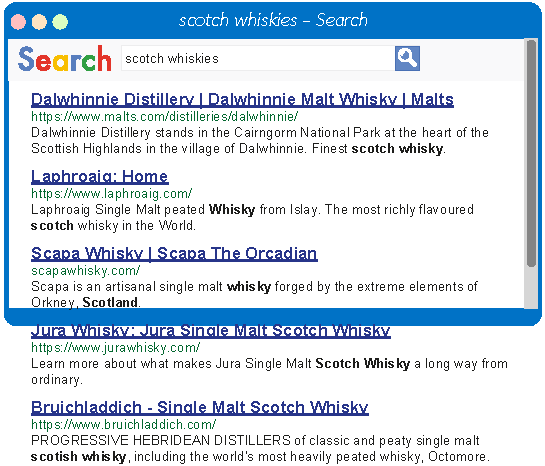
\includegraphics[width=1\textwidth]{figures/ch6-viewport.pdf}
    \end{center}
    \vspace*{-2mm}
    \caption[Viewport cutoff example]{The~\gls{acr:serp} viewport threshold. In this example, three result summaries are visible, with two present but outwith the viewport. Therefore, \emph{v\textsubscript{size}=3}.}
    \label{fig:viewport_cutoff}
\end{wrapfigure}

We argue that a searcher can infer the quality of the~\gls{acr:serp} from the initial view with which they are presented, and thus incorporate a \emph{viewport size} ($v_{size}$) variable in our simulations of interaction -- a searcher can only judge what they can see. This variable can vary between the different interfaces we trialled. For example, longer snippet text resulted in fewer result summaries being displayed in the initial view. By using a fixed-size popup window in the two user studies (as discussed in Section~\ref{sec:methodology:user:interface}), we were able to manually check the number of result summaries displayed within the popup window, and use these values to provide more extensive grounding to the new stopping decision point.

For simulations of interaction reported in Chapter~\ref{chap:snippets}, different values of $v_{size}$ could be used over the four experimental interfaces trialled. This was because for each interface, result summary lengths varied. As we tended from interface \blueboxbold{T0} (no snippet text) to \blueboxbold{T4} (four snippet fragments), longer result summaries would impact upon the number of result summaries visible in the initial view. Longer result summaries would mean that fewer would be presented within a viewport of the same size, compared to shorter result summaries. However, result summary lengths were not modified under the experimental conditions trialled in Chapter~\ref{chap:diversity}. This means that $v_{size}$ would (on average) remain constant, with fixed popup window dimensions resulting in two lines of snippet text per result summary.

\blueboxbold{Definition: Low vs. High Scent} Given a~\gls{acr:serp}, would it constitute as \emph{low scent} or \emph{high scent?} For this chapter, we follow the work of~\cite{wu2014information_scent}. In their study, the authors state that a low scent~\gls{acr:serp} offers little or no relevant content. Definitions by~\cite{wu2014information_scent} and~\cite{hassan2013serp_abandonment} define a poor scented~\gls{acr:serp} as $P@10=0.0$. We take this definition to delineate between \emph{good} and \emph{bad}~\glsplural{acr:serp}, and extend it by also considering $v_{size}$. This leads to our definition of $P@v_{size}=0.0$ for a poor quality~\gls{acr:serp}, meaning that a simulated searcher would then gauge the quality of a~\gls{acr:serp} by examining the average number of result summaries displayed within a fictional browser viewport for the given experimental interface or condition being trialled. The definition of low and high scented~\glsplural{acr:serp} was also used for \blueboxbold{SS11-COMB}, as defined in Section~\ref{sec:strategies:time} on page~\pageref{sec:strategies:time}.

\blueboxbold{Probability of Examination} For this new stopping decision point, we introduce the \emph{probability of examining a~\gls{acr:serp}}, or \blueboxbold{P(E)}. This determines how likely it is that a searcher will \emph{enter} a~\gls{acr:serp} and begin to examine result summaries in detail. Taking this concept further, we can then consider two further probabilities of interaction that incorporate the notion of a~\glsplural{acr:serp} information scent, yielding:

\begin{itemize}
    \item{\blueboxbold{P(E|HS)}, the probability of examining a~\gls{acr:serp} perceived to give a high information scent (i.e. a good quality~\gls{acr:serp}); and}
    \item{\blueboxbold{P(E|LS)}, the probability of examining a~\gls{acr:serp} offering what appears to be a low information scent (i.e. a poor quality~\gls{acr:serp}, or $P@v_{size}=0.0$).}
\end{itemize}

\begin{figure}[t!]
    \centering
    \resizebox{1\hsize}{!}{
    
\includegraphics{figures/ch6-serp_probabilities.pdf}}
    \caption[Computing~\gls{acr:serp} examination probabilities]{An illustration highlighting how the different~\gls{acr:serp} examination costs were computed. As an example, low scented~\glsplural{acr:serp} offering \emph{P@v\textsubscript{size} = 0.0} are selected, with the calculation for \emph{P(E|LS)} then taking place. We consider both the probability of examining~\glsplural{acr:serp} yielding both high and low information scents. The definitions for low and high scented~\glsplural{acr:serp} using \emph{v\textsubscript{size}} are adapted from~\cite{wu2014information_scent} and~\cite{hassan2013serp_abandonment}.}
    \label{fig:serp_probabilities}
\end{figure}

These values were computed from interaction log data, taken from the two user studies reported in Chapters~\ref{chap:snippets} and~\ref{chap:diversity}. Computed values derived are not reported in this section; refer to Section~\ref{sec:serp:method:probscosts} for the probabilities. Intuitively, one would expect a searcher demonstrating competency at searching for information to know when a query is returning good results and vice versa. As such, one would expect to see a higher probability for $P(E|HS)$ than when compared to $P(E|LS)$, and would provide evidence that searchers do indeed attempt to avoid low quality~\glsplural{acr:serp}.

As illustrated in Figure~\ref{fig:serp_probabilities}, we took each query issued from the interaction log of each user study, and extracted for each the $P@v_{size}$ score (as per~\cite{wu2014information_scent}), considering $P@v_{size}=0.0$ as our criterion for a~\gls{acr:serp} of poor scent. For the interactions recorded on each~\gls{acr:serp}, we could then count the number that recorded no clicks (meaning no result summaries were deemed to be attractive enough to examine further). We considered this as a definition of an \blueboxbold{abandoned~\gls{acr:serp}}, as used in previous work by~\cite{hassan2013serp_abandonment}. From these counts, we could then compute the probabilities of examining a~\gls{acr:serp}, as illustrated in Figure~\ref{fig:serp_probabilities}.

\subsubsection{Decision Point Implementations}\label{sec:serp:method:serp_dp:implementations}
We trialled three different implementations of the~\gls{acr:serp} level stopping decision point, providing us with the ability to explore the effect of incorporating it within the~\gls{acr:csm}. These are enumerated below, with an explanation of each. The first can be considered our baseline approach.

\begin{itemize}
    \item{\dualbluebox{SERP}{Always} Considered our baseline, a searcher subscribing to this implementation will always enter the~\gls{acr:serp} and examine at least one result summary -- the exact number would be determined by the result summary level stopping strategy. This is the generally accepted approach as used in prior simulations of interaction. As such, we consider this to be our baseline implementation. As a reminder, this implementation was used in the simulations reported in Chapters~\ref{chap:snippets} and~\ref{chap:diversity}.}
\end{itemize}

From here, the remaining two strategies begin to consider a simulated searcher's judgements regarding the perceived quality of a~\gls{acr:serp}, and thus begin to use the new stopping decision point to abandon a~\gls{acr:serp} before examining individual result summaries in detail.

\begin{itemize}
    \item{\dualbluebox{SERP}{Perfect} Here, a simulated searcher will only begin to examine a~\gls{acr:serp} in detail if $P@v_{size} > 0$ (considering the viewport size). If $P@v_{size} = 0$, the searcher will abandon the~\gls{acr:serp}, and proceed to the next action as dictated by the~\gls{acr:csm}. This is the upper bound in terms of performance for the stopping decision point, and is analogous to, as an example, the \emph{ideal user} of~\cite{hagen2016simulating_users}.}
    
    \item{\dualbluebox{SERP}{Average} This final implementation used a stochastic element to determine whether the simulated searcher should enter the~\gls{acr:serp} or not. Like above, the viewport size ($P@v_{size}$) of the~\gls{acr:serp} is computed. If the~\gls{acr:serp} is of high scent, $P(E|HS)$ is used to determine whether the searcher should enter the~\gls{acr:serp}. Conversely, if the~\gls{acr:serp} is considered to be of low scent, $P(E|LS)$ is used instead to determine the likelihood of abandonment. We considered the probabilities of interaction for a given interface or condition, taking the average.}
    
%      We considered three different sets of probabilities for the stochastic implementation.}
%
%     \begin{itemize}
%         \item{\blueboxbold{Average} $P(E|HS)$ and $P(E|LS)$ are estimated over all subjects of a particular interface or condition.}
%         \item{\blueboxbold{Savvy} $P(E|HS)$ and $P(E|LS)$ are estimated based upon the top 15 subjects for a particular interface/condition with the \emph{lowest} $P(E|LS)$.}
%         \item{\blueboxbold{Na\"{i}ve} $P(E|HS)$ and $P(E|LS)$ are estimated based upon the top 15 subjects for a particular interface/condition with the \emph{highest} $P(E|LS)$.}
%     \end{itemize}
\end{itemize}

Given the three implementations, one would intuitively expect \dualbluebox{SERP}{Perfect} to yield simulated searcher that attain the highest overall levels of~\gls{acr:cg}. These searchers would not waste time examining poor scented~\glsplural{acr:serp}, and instead spend their time examining~\glsplural{acr:serp} that will return at least one relevant document. For the implementation that offers the best approximations of real-world stopping behaviours however, \dualbluebox{SERP}{Perfect} may not be best. It depends how well real-world subjects were able to discern from good and poor scented~\glsplural{acr:serp}. It is more likely that \dualbluebox{SERP}{Average} will provide the better approximations of real-world behaviours.

By considering the three different approaches to implementing the new~\gls{acr:serp} level stopping decision point, we can then clearly identify whether improved performance and improved approximations of actual searcher stopping behaviours are offered. We also trialled each of the stochastic~\gls{acr:serp} level stopping decision components a total of 10 times, computing the average over the different trials. Given that the decision maker components of the \simiir~framework were run a total of 50 times each (responsible for determining the attractiveness of result summaries and relevancy of documents), this made the addition of a stochastic~\gls{acr:serp} level stopping decision point expensive in terms of the additional runs required.

%A larger number of trials would have been prohibitive (primarily in terms of execution time required) given the apparatus available for the simulations.

\subsection{Interfaces, Conditions, and Experimental Grounding}\label{sec:serp:method:probscosts}
To determine whether the new~\gls{acr:serp} level stopping decision point implementations offered improvements, we conducted a series of simulations across interfaces and conditions trialled in the two user studies, reported earlier in Chapters~\ref{chap:snippets} and~\ref{chap:diversity}.

From Chapter~\ref{chap:snippets}, the four different experimental interfaces -- whereby result summary lengths were manipulated -- were considered. Namely, these were \blueboxbold{T0}, \blueboxbold{T1}, \blueboxbold{T2} and \blueboxbold{T4}. From Chapter~\ref{chap:diversity}, we also considered the four experimental conditions that manipulated the underlying system and searcher tasks: \dualbluebox{D}{AS}, \dualbluebox{ND}{AS}, \dualbluebox{D}{AD} and \dualbluebox{ND}{AD}.

\begin{table}[t!]
    \caption[\emph{P(E|HS)} and \emph{P(E|LS)} probabilities, with v\textsubscript{size}]{Probabilities of examining high (\genericblack{P(E|HS)}) and low scented~\glsplural{acr:serp} (\genericblack{P(E|LS)}), along with \genericblack{v\textsubscript{size}} values for each of the experimental interfaces and conditions trialled in this chapter. Statistical tests between interfaces/conditions yielded no significant differences, at $\alpha$\emph{=0.05.} Probabilities that are used in the experiments reported in this chapter are \darkbluebox{highlighted.} Refer to Tables~\ref{tbl:snippets_simulation_probcosts} (page~\pageref{tbl:snippets_simulation_probcosts}) and~\ref{tbl:diversity_simulation_probcosts} (page~\pageref{tbl:diversity_simulation_probcosts}) for other interaction probabilities and costs for the studies reported in Chapters~\ref{chap:snippets} and~\ref{chap:diversity}.}
    \label{tbl:serp_probs_costs}
    \renewcommand{\arraystretch}{1.8}
    \begin{center}
    \begin{tabulary}{\textwidth}{L{0.1cm}@{\CS}L{3.875cm}@{\CS}D{2.4cm}@{\CS}D{2.4cm}@{\CS}D{2.4cm}@{\CS}D{2.4cm}@{\CS}}

        \RS & & \lbluecell \textbf{T0} & \lbluecell \textbf{T1} & \dbluecell \textbf{T2} & \lbluecell \textbf{T4} \\
        
        \RS \multirow{3}{*}{\hspace*{-2mm}\rotatebox{90}{\hspace*{-7mm} Chapter~\ref{chap:snippets}}} & \lbluecell\textbf{P(E|HS)} & \cell \small{0.76} & \cell \small{0.79} & \dbluecell \small{0.78} & \cell \small{0.78}\\
        \RS & \lbluecell\textbf{P(E|LS)} & \cell \small{0.27} & \cell \small{0.40} & \dbluecell \small{0.31} & \cell \small{0.40}\\
        %
        % % \RS\RS\RS \multirow{2}{*}{\rotatebox{90}{\hspace*{-2mm}\textbf{Savvy}}} & \lbluecell\textbf{P(E|HS)} & \cell \small{0.69} & \cell \small{0.86} & \cell \small{0.83} & \cell \small{0.82}\\
        % % \RS & \lbluecell\textbf{P(E|LS)} & \cell \small{0.00} & \cell \small{0.00} & \cell \small{0.00} & \cell \small{0.00}\\
        % %
        % % \RS\RS\RS \multirow{2}{*}{\rotatebox{90}{\hspace*{-2mm}\textbf{Na\"{i}ve}}} & \lbluecell\textbf{P(E|HS)} & \cell \small{0.48} & \cell \small{0.53} & \cell \small{0.52} & \cell \small{0.53}\\
        % % \RS & \lbluecell\textbf{P(E|LS)} & \cell \small{0.16} & \cell \small{0.30} & \cell \small{0.23} & \cell \small{0.25}\\
        %
        \RS\RS\RS & \lbluecell\textbf{v\textsubscript{size}} & \cell \small{10} & \cell \small{9} & \dbluecell \small{7} & \cell \small{6}\\
        %
        \RS\RS\RS\RS\RS\RS & & \lbluecell \textbf{D-AS} & \lbluecell \textbf{ND-AS} & \lbluecell \textbf{D-AD} & \dbluecell \textbf{ND-AD} \\
        %
        \RS \multirow{3}{*}{\hspace*{-2mm}\rotatebox{90}{\hspace*{-7mm} Chapter~\ref{chap:diversity}}} & \lbluecell\textbf{P(E|HS)} & \cell \small{0.76} & \cell \small{0.76} & \cell \small{0.73} & \dbluecell \small{0.75}\\
        \RS & \lbluecell\textbf{P(E|LS)} & \cell \small{0.29} & \cell \small{0.37} & \cell \small{0.26} & \dbluecell \small{0.34}\\
        %
        % % \RS\RS\RS \multirow{2}{*}{\rotatebox{90}{\hspace*{-2mm}\textbf{Savvy}}} & \lbluecell\textbf{P(E|HS)} & \cell \small{0.77} & \cell \small{0.75} & \cell \small{0.89} & \cell \small{0.78}\\
        % % \RS & \lbluecell\textbf{P(E|LS)} & \cell \small{0.00} & \cell \small{0.37} & \cell \small{0.00} & \cell \small{0.30}\\
        % %
        % % \RS\RS\RS \multirow{2}{*}{\rotatebox{90}{\hspace*{-2mm}\textbf{Na\"{i}ve}}} & \lbluecell\textbf{P(E|HS)} & \cell \small{0.57} & \cell \small{0.52} & \cell \small{0.41} & \cell \small{0.54}\\
        % % \RS & \lbluecell\textbf{P(E|LS)} & \cell \small{0.31} & \cell \small{0.37} & \cell \small{0.24} & \cell \small{0.35}\\
        %
        \RS\RS\RS & \lbluecell\textbf{v\textsubscript{size}} & \cell \small{7} & \cell \small{7} & \cell \small{7} & \dbluecell \small{7}\\
        
    \end{tabulary}
    \end{center}
\end{table}

From the interaction data of the two user study interaction logs, we could then compute the probabilities of subjects examining low scented ($P(E|LS)$) and high scented ($P(E|HS)$)~\glsplural{acr:serp}. Values were computed as per the explanations provided in Section~\ref{sec:serp:method:serp_dp}. The computed values are reported in Table~\ref{tbl:serp_probs_costs}, along with the corresponding $v_{size}$ value for each interface or condition, denoting the number of result summaries visible within a simulated viewport. From examination of the table, we can see that the probabilities for both sets are very similar across all interfaces and conditions. Indeed, a two-tailed Student's t-test yielded no significant differences across the four interfaces or conditions where $\alpha=0.05$. Given the close proximity of the probabilities (and the subsequent lack of differences that we would likely observe), we simplified our experimentation. We chose to run experiments for one interface and condition per study, selecting \blueboxbold{T2} and \dualbluebox{ND}{AD}. These were selected as they represent a standard search interface and task.

Values reported in Table~\ref{tbl:serp_probs_costs} should be considered in tandem with the interaction costs and probabilities reported in Tables~\ref{tbl:snippets_simulation_probcosts} (page~\pageref{tbl:snippets_simulation_probcosts}) and~\ref{tbl:diversity_simulation_probcosts} (page~\pageref{tbl:diversity_simulation_probcosts}). These tables report interaction costs (such as querying and document examination costs) and other probabilities (considering the probabilities of clicking on result summaries, $P(C|R)$ and $P(C|N)$ -- and saving documents, $P(S|R)$ and $P(S|N)$).

%Values reported in Table~\ref{tbl:serp_probs_costs} should be considered in tandem with the interaction costs and probabilities presented in Tables~\ref{tbl:snippets_simulation_probcosts} (presented on page~\pageref{tbl:snippets_simulation_probcosts}) and~\ref{tbl:diversity_simulation_probcosts} (presented on page~\pageref{tbl:diversity_simulation_probcosts}) for other interaction probabilities (considering the probabilities of considering the attractiveness of result summaries, $P(C|R)$ and $P(C|N)$ -- and saving documents, $P(S|R)$ and $P(S|N)$) and interaction costs (including the cost of: querying; examining a~\gls{acr:serp}; examining a result summary; examining a document; and saving a document) for the studies reported in Chapters~\ref{chap:snippets} and~\ref{chap:diversity} respectively.

% Table~\ref{tbl:serp_probs_costs} presents the probabilities of examining~\glsplural{acr:serp} yielding low ($P(E|LS)$) and high ($P(E|HS)$) scents. Values are computed as per the explanations provided in Section~\ref{sec:serp:method:serp_dp}. The table reports values across each of the eight different experimental interfaces and conditions trialled. In addition, values are reported for each interface and condition across the three different probability sets of \emph{average, savvy} and \emph{na\"{i}ve} searchers (as discussed in Section~\ref{sec:serp:method:serp_dp:implementations}). Also included within the table are the $v_{size}$ values used across each interface or condition, denoting the number of result summaries visible within a simulated viewport. Note the interaction probabilities that are conducive to \emph{savvy} or \emph{na\"{i}ve}~\gls{acr:serp} examination behaviour -- across interfaces \blueboxbold{T0}, \blueboxbold{T1}, \blueboxbold{T2} and \blueboxbold{T4}, searchers will never examine a~\gls{acr:serp} of low scent. In contrast, the likelihood of examining a~\gls{acr:serp} of poor scent increases from a zero chance to the region of $16\%$ to $30\%$ for na\"{i}ve searchers.

% These values should be considered in tandem with the interaction costs and probabilities presented in Tables~\ref{tbl:snippets_simulation_probcosts} (presented on page~\ref{tbl:snippets_simulation_probcosts}) and~\ref{tbl:diversity_simulation_probcosts} (presented on page~\pageref{tbl:diversity_simulation_probcosts}) for other classical interaction probabilities (considering the probabilities of marking result summaries, $P(C|R)$ and $P(C|N)$ -- and saving documents, $P(S|R)$ and $P(S|N)$) and interaction costs (including the cost of: querying; examining a~\gls{acr:serp}; examining a result summary; examining a document; and saving a document) for the studies reported in Chapters~\ref{chap:snippets} and~\ref{chap:diversity} respectively. Table~\ref{tbl:serp_probs_costs} reports only the probabilities of examining a~\gls{acr:serp}.

\subsection{Result Summary Level Stopping Strategies}\label{sec:serp:method:snippet}
Chapter~\ref{chap:strategies} presented twelve different result summary level stopping strategies. To further reduce the complexity of the experimentation reported in this chapter, we decided to reduce the number of strategies that we considered. Doing so reduced the risk of potentially repeating the same results as shown before, while still demonstrating that when enabled, the~\gls{acr:serp} level stopping decision point yielded improved performance (and closer approximations) to actual searcher stopping behaviour -- while still reporting over a range of configurations.

We only report the results of three result summary level stopping strategies in this chapter. These were selected as they offered good performance and approximations of actual searcher stopping behaviours in results presented in previous chapters. We used:

\begin{itemize}
    \item{\blueboxbold{SS1-FIX}, the fixed-depth baseline result summary level stopping strategy;}
    \item{\blueboxbold{SS2-NT}, the frustration stopping strategy, considering the total number of non-relevant summaries encountered; and}
    \item{\blueboxbold{SS5-COMB}, the combination stopping strategy combining frustration-based strategy \blueboxbold{SS2-NT} and satisfaction-based strategy \blueboxbold{SS4-SAT}.}
\end{itemize}

Definitions for each of these stopping strategies can be found in Chapter~\ref{chap:strategies}, starting on page~\pageref{chap:strategies}. Note that these strategies were instantiated with the same $x_n$ values \emph{(stopping threshold values)} reported in the general methodology in Section~\ref{sec:method:simulation:grounding:stopping} (page~\pageref{sec:method:simulation:grounding:stopping}).

\subsection{Remaining CSM Components}\label{sec:serp:method:other}
The remaining~\gls{acr:csm} components were configured as presented in Section~\ref{sec:method:simulation:runs:performance}. For comparison runs, queries issued by real-world subjects under \blueboxbold{T2} and \dualbluebox{ND}{AD} were again \emph{replayed} in the simulations, the process of which is outlined in Section~\ref{sec:method:simulation:runs:comparison} on page~\pageref{sec:method:simulation:runs:comparison}. Specific implementation details for interface \blueboxbold{T2} were the same as described in Section~\ref{sec:snippets:simulations:method} (page~\pageref{sec:snippets:simulations:method}), with the methodology in Section~\ref{sec:diversity:simulated:method} (page~\pageref{sec:diversity:simulated:method}) followed for \dualbluebox{ND}{AD}.

%
% For the four experimental interfaces trialled in the study reported in Chapter~\ref{chap:snippets}, the same experimental methodology was followed as described in Section~\ref{sec:snippets:simulations:method}. Similarly, the same experimental method was followed as reported in Section~\ref{sec:diversity:simulated:method} for the four experimental conditions belonging to the studies reported in Chapter~\ref{chap:diversity}. This involved, for example, executing the diversification algorithm (presented in Section~\ref{sec:diversity:users:diversifying} on page~\pageref{sec:diversity:users:diversifying}) over the ranked results returned for the diversified system, \blueboxbold{D}.

\section{Results}\label{sec:serp:results}
We now report the results of our simulations of interaction, involving the new~\gls{acr:serp} level stopping decision point. As in previous chapters, we discuss our findings over two subsections, considering:

\begin{itemize}
    \item{\blueboxbold{performance runs} (Section~\ref{sec:serp:results:perf}), where we discuss the highest levels of performance attained by simulated searchers under different \emph{what-if} scenarios; and}
    \item{\blueboxbold{comparison runs} (Section~\ref{sec:serp:results:comparisons}), where we provide results of the simulations that were directly compared to actual mean searcher stopping behaviours.}
\end{itemize}

Both of these runs provide answers for this chapter's two research questions, \darkblueboxbold{SERP-RQ1} and \darkblueboxbold{SERP-RQ2}. Refer to Section~\ref{sec:serp:background} for information on the questions posed.

\blueboxheader{Significance Testing}
While the difference between individual result summary level stopping strategies is interesting, the main focus of the results reported in this chapter is the difference in performance and approximations offered across individual~\gls{acr:serp} level decision point implementations. Statistical tests in this chapter are therefore performed across different~\gls{acr:serp} level decision point implementations to determine if significant differences exist between them. All tests reported in this chapter utilise the two-tailed Student's t-test, where $\alpha=0.05$. Unlike Sections~\ref{sec:snippets:simulations} and~\ref{sec:diversity:simulated}, we this time examine results \emph{for} significant differences between the implementations.

\subsection{Performance}\label{sec:serp:results:perf}
Figure~\ref{fig:ch9_perf_plots} presents six individual plots, each representing one of the three different result summary level stopping strategies trialled (from \blueboxbold{SS1-FIX}, \blueboxbold{SS2-NT} and \blueboxbold{SS5-COMB}). The three plots on the top correspond to results over interface \blueboxbold{T2} (Chapter~\ref{chap:snippets}), with the bottom three plots corresponding to condition \dualbluebox{ND}{AD} (Chapter~\ref{chap:diversity}). Each plot represents the mean level of~\gls{acr:cg} that is attained across the runs (represented on the $y$ axes) across varying mean depths per query (along the $x$ axes). In each plot, we represent the three individual~\gls{acr:serp} level stopping decision points, with our baseline \dualbluebox{SERP}{Always}, \dualbluebox{SERP}{Average} and \dualbluebox{SERP}{Perfect} presented. This means that we can observe how performance varies across different depths, over different result summary level stopping strategies -- and over a different interface/condition.

\begin{figure}[t!]
    \centering
    \resizebox{1\hsize}{!}{
    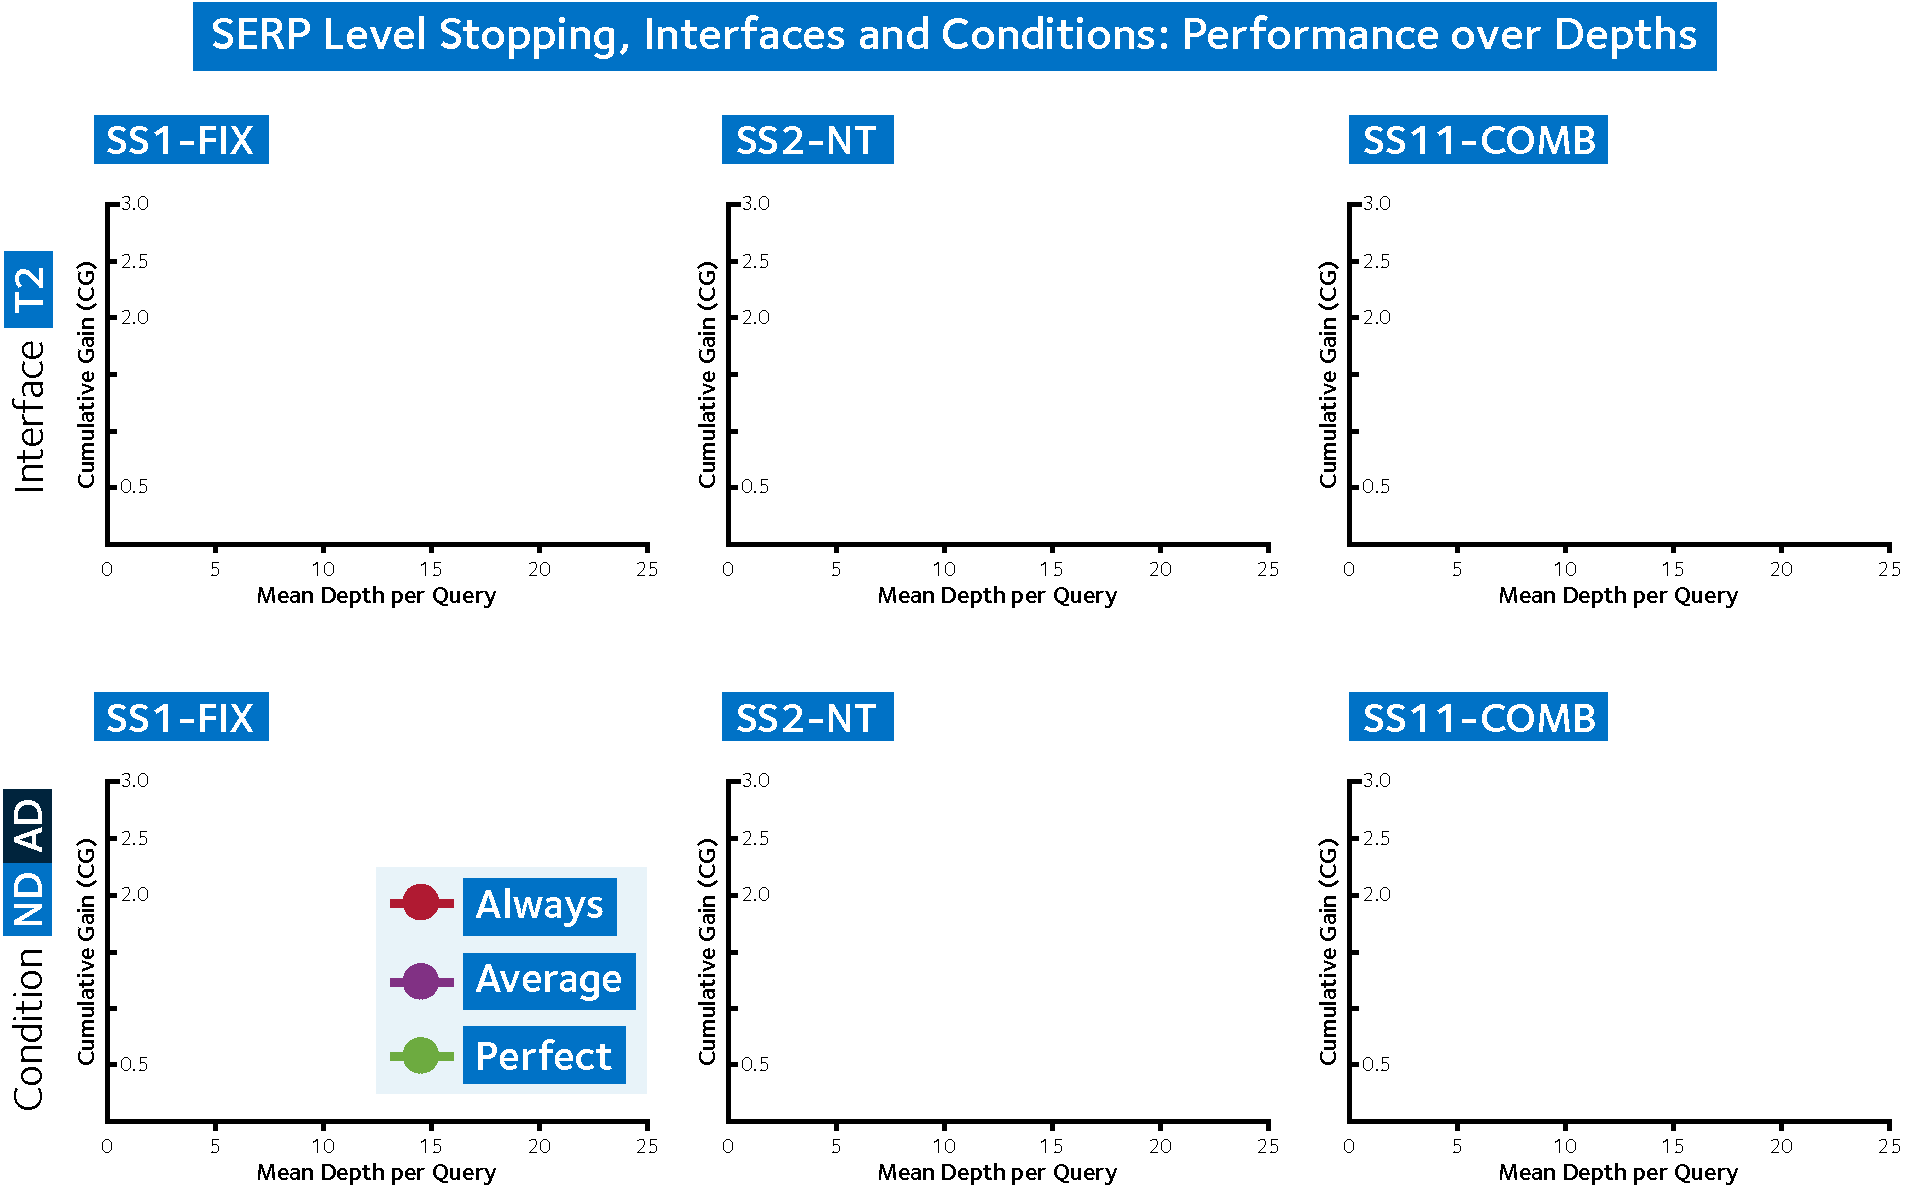
\includegraphics{figures/ch9-perf_plots.pdf}}
    \caption[Stopping strategies and~\gls{acr:serp} decision point \emph{what-if} performance]{Plots demonstrating the varying levels of performance, measured in~\gls{acr:cg}, over the mean depth per query. Plots are for the \emph{what-if} simulated performance runs. Each result summary level stopping strategy is plotted separately, with the three different~\gls{acr:serp} level decision point implementations shown. Plots on the top relate to interface \blueboxbold{T2}; plots on the bottom relate to condition \dualbluebox{ND}{AD}.}
    \label{fig:ch9_perf_plots}
\end{figure}

From an initial observation of the plots, we note a number of different (and consistently occurring) trends. As with the plots in Figures~\ref{fig:ch7_sim_perf_plots} (page~\pageref{fig:ch7_sim_perf_plots}) and~\ref{fig:ch8_sim_perf_plots} (page~\pageref{fig:ch8_sim_perf_plots}), we observe that at low mean depths per query, all three~\gls{acr:serp} level decision point implementations offer similar levels of~\gls{acr:cg}.~\gls{acr:cg} then steadily rises up to a peak as the mean depth per query increases. Once this peak has been reached, the performance then begins to slowly tail off, or remain relatively invariant across greater mean depths per query. Of particular relevance to \darkblueboxbold{SERP-RQ1} is the difference in~\gls{acr:cg} attained by the three different~\gls{acr:serp} level stopping decision point implementations. As previously mentioned, all three start from a similar point at shallow depths per query, across all stopping strategies and the interface/condition. However, as the mean depth per query increases, we observe that the performance across the three different implementations begins to diverge from one another.

We consistently find that as the mean depth per query increases, the \dualbluebox{SERP}{Always} (baseline) implementation consistently offers the lowest levels of~\gls{acr:cg}, and the \dualbluebox{SERP}{Perfect} implementation consistently offers higher levels of mean~\gls{acr:cg}. This is an intuitive result; avoiding~\glsplural{acr:serp} that offer a poor scent means that you are likely to invest more time in issuing queries that offer better results, thus identifying and saving more relevant documents. This consistent improvement also provides evidence for addressing \darkblueboxbold{SERP-RQ1} -- incorporating a~\gls{acr:serp} level stopping decision point does indeed lead to higher overall performance. The final implementation \dualbluebox{SERP}{Average} presents further evidence to support this claim, with performance generally performing better than the baseline \dualbluebox{SERP}{Always} implementation. However, it should be noted that there are certain points where \dualbluebox{SERP}{Always} does outperform \dualbluebox{SERP}{Average}. For example, examining the plot in Figure~\ref{fig:ch9_perf_plots} for interface \blueboxbold{T2} over stopping strategy \blueboxbold{SS2-NT}, one can see that \dualbluebox{SERP}{Always} outperforms \dualbluebox{SERP}{Average} at a mean depth per query from around $6$ to $8$. This may be because that a simulated searcher may decide to skip some queries judged to yield a poor scented~\gls{acr:serp}, and would therefore have the time to issue more queries later on in the session. As we do not consider previously examined content in the initial~\gls{acr:serp} judgement, a simulated searcher may enter subsequent~\glsplural{acr:serp} without any additional relevant content to mark, lowering their overall mean~\gls{acr:cg}. We discuss this potential limitation later in Chapter~\ref{chap:conclusions}.

\begin{table}[t!]
    \caption[Maximum~\gls{acr:cg} from \emph{what-if} performance runs]{Results from the simulated \emph{what-if} simulated performance runs, showing the highest levels of~\gls{acr:cg} attained for result summary level stopping strategies \blueboxbold{SS1-FIX}, \blueboxbold{SS2-NT} and \blueboxbold{SS5-COMB}. These are reported over the \dualbluebox{SERP}{Always} \emph{(baseline),} \dualbluebox{SERP}{Average} and \dualbluebox{SERP}{Perfect}~\gls{acr:serp} level stopping decision point implementations. \genericblack{x\textsubscript{n}} denotes the stopping parameter threshold(s), with \genericblack{DQ} denoting the depth per query at which the greatest \genericblack{\gls{acr:cg}} value was attained at. Note that for combination strategy \blueboxbold{SS5-COMB}, \emph{x\textsubscript{2},x\textsubscript{4}} are shown as \genericblack{x\textsubscript{n}} column. Stopping strategy/\gls{acr:serp} decision point implementation combinations that yield the highest~\gls{acr:cg} values are \darkbluebox{highlighted}.}
    \label{tbl:ch9_perf_table}
    \renewcommand{\arraystretch}{1.8}
    \begin{center}
        \begin{tabulary}{\textwidth}{L{0.25cm}@{\CS}L{2.18cm}@{\CS}D{0.895cm}@{\CS}D{0.895cm}@{\CS}D{0.895cm}@{\CSONEHALF}D{0.895cm}@{\CS}D{0.895cm}@{\CS}D{0.895cm}@{\CSONEHALF}D{0.895cm}@{\CS}D{0.895cm}@{\CS}D{0.895cm}@{\CSONEHALF}}
            
            & & \multicolumn{3}{@{\hskip 0pt}c@{\CSONEHALF}}{\dbluecell\small\textbf{Always}} & \multicolumn{3}{@{\hskip 0pt}c@{\CSONEHALF}}{\dbluecell\small\textbf{Average}} & \multicolumn{3}{@{\hskip 0pt}c@{\CSONEHALF}}{\dbluecell\small\textbf{Perfect}}\\
            
            \RS & & \lbluecell\small\textbf{x\textsubscript{n}} & \lbluecell\small\textbf{DQ} & \lbluecell\small\textbf{CG} & \lbluecell\small\textbf{x\textsubscript{n}} & \lbluecell\small\textbf{DQ} & \lbluecell\small\textbf{CG} & \lbluecell\small\textbf{x\textsubscript{n}} & \lbluecell\small\textbf{DQ} & \lbluecell\small\textbf{CG} \\
            
            % T2
            \RS \multirow{3}{*}{\hspace*{-2mm}\rotatebox{90}{\hspace*{-7mm}\footnotesize Int. \blueboxbold{\textbf{T2}}}} & \lbluecell\small\textbf{SS1-FIX} & \cell \small \hspace*{-1mm} 10 & \cell \small \hspace*{-1mm} 6.33 & \cell \hspace*{-1mm} \small 2.50 & \cell \small \hspace*{-1mm} 10 & \cell \small \hspace*{-1mm} 4.17 & \cell \hspace*{-1mm} \small 2.45 & \cell \small \hspace*{-1mm} 10 & \cell \small \hspace*{-1mm} 4.45 & \dbluecell \hspace*{-1mm} \small 2.98 \\
            \RS  & \lbluecell\small\textbf{SS2-NT} & \cell \small \hspace*{-1mm} 7 & \cell \small \hspace*{-1mm} 6.16 & \cell \hspace*{-1mm} \small 2.49 & \cell \small \hspace*{-1mm} 21 & \cell \small \hspace*{-1mm} 10.77 & \cell \hspace*{-1mm} \small 2.58 & \cell \small \hspace*{-1mm} 8 & \cell \small \hspace*{-1mm} 5.07 & \dbluecell \hspace*{-1mm} \small 3.11 \\
            \RS  & \lbluecell\small\textbf{SS5-COMB} & \cell \small \hspace*{-1mm} 8,4 & \cell \small \hspace*{-1mm} 6.17 & \cell \hspace*{-1mm} \small 2.52 & \cell \small \hspace*{-1mm} 21,9 & \cell \small \hspace*{-1mm} 10.54 & \cell \hspace*{-1mm} \small 2.59 & \cell \small \hspace*{-1mm} 8,7 & \cell \small \hspace*{-1mm} 5.04 & \dbluecell \hspace*{-1mm} \small 3.14 \\
            
            % ND-AD
            \RS\RS\RS \multirow{3}{*}{\hspace*{-2mm}\rotatebox{90}{\hspace*{-7mm}\footnotesize Cdn. \textbf{\dualbluebox{ND}{AD}}}} & \lbluecell\small\textbf{SS1-FIX} & \cell \small \hspace*{-1mm} 10 & \cell \small \hspace*{-1mm} 6.47 & \cell \hspace*{-1mm} \small 1.81 & \cell \small \hspace*{-1mm} 10 & \cell \small \hspace*{-1mm} 3.93 & \cell \hspace*{-1mm} \small 1.82 & \cell \small \hspace*{-1mm} 10 & \cell \small \hspace*{-1mm} 4.69 & \dbluecell \hspace*{-1mm} \small 2.30 \\
            \RS  & \lbluecell\small\textbf{SS2-NT} & \cell \small \hspace*{-1mm} 10 & \cell \small \hspace*{-1mm} 7.55 & \cell \hspace*{-1mm} \small 1.80 & \cell \small \hspace*{-1mm} 10 & \cell \small \hspace*{-1mm} 4.71 & \cell \hspace*{-1mm} \small 1.84 & \cell \small \hspace*{-1mm} 5 & \cell \small \hspace*{-1mm} 3.12 & \dbluecell \hspace*{-1mm} \small 2.35 \\
            \RS  & \lbluecell\small\textbf{SS5-COMB} & \cell \small \hspace*{-1mm} 10,6 & \cell \small \hspace*{-1mm} 7.55 & \cell \hspace*{-1mm} \small 1.80 & \cell \small \hspace*{-1mm} 10,4 & \cell \small \hspace*{-1mm} 4.43 & \cell \hspace*{-1mm} \small 1.85 & \cell \small \hspace*{-1mm} 10,3 & \cell \small \hspace*{-1mm} 4.87 & \dbluecell \hspace*{-1mm} \small 2.37 \\

        \end{tabulary}
        \end{center}
    \end{table}

Given the evidence supporting \darkblueboxbold{SERP-RQ1}, we now turn our attention to the absolute best performance that each of the stopping strategies yield, across each interface/condition and over the three~\gls{acr:serp} level stopping decision point implementations. Table~\ref{tbl:ch9_perf_table} provides these values, with values for interface \blueboxbold{T2} reported first, and condition \dualbluebox{ND}{AD} reported underneath. For each stopping strategy and~\gls{acr:serp} level stopping decision point combination, we report: the highest level of \genericblack{CG} attained; the mean depth per query (\genericblack{DQ}) that this was attained at, and the stopping threshold(s) (\genericblack{x\textsubscript{n}}) that were used. For combination stopping strategy \blueboxbold{SS5-COMB}, two stopping threshold values were used for $x_2$ and $x_4$. These are presented in Table~\ref{tbl:ch9_perf_table} in this order.

From Table~\ref{tbl:ch9_perf_table}, we find results that complement the findings observed in Figure~\ref{fig:ch9_perf_plots}. In the table, we \darkbluebox{highlight} the~\gls{acr:serp} level stopping decision point implementation and stopping strategy combination yielding the highest level of mean~\gls{acr:cg}. Unsurprisingly, these are all obtained with the \dualbluebox{SERP}{Perfect}~\gls{acr:serp} level stopping decision point implementation. Indeed, a general trend from the table can be observed -- improvements in the highest levels of~\gls{acr:cg} can be clearly seen as we tend from left to right, or \dualbluebox{SERP}{Always} to \dualbluebox{SERP}{Perfect}. The biggest increase in maximum~\gls{acr:cg} that can be observed from the table is for \blueboxbold{SS5-COMB} over interface \blueboxbold{T2}, with mean~\gls{acr:cg} rising from $2.52$ and a mean depth per query of $6.17$ to $3.14$, at a mean depth per query of $5.04$. Interestingly, the rises in~\gls{acr:cg} are more profound over \blueboxbold{T2} generally when compared to the results obtained over condition \dualbluebox{ND}{AD}.

Closer inspection of the values reported for the \dualbluebox{SERP}{Always}~\gls{acr:serp} level stopping decision point implementation reported in Table~\ref{tbl:ch9_perf_table} can also be undertaken. These values are considered as our initial baseline, and are essentially the values attained by the simulated searchers when instructed to browse every resultant~\gls{acr:serp}. As such, this is the configuration that is employed in the results of the simulations of interaction we presented in Chapters~\ref{chap:snippets} and~\ref{chap:diversity}. Specifically, values of interface \blueboxbold{T2} reported in Table~\ref{tbl:ch7_sim_perf} on page~\pageref{tbl:ch7_sim_perf} match those reported in Table~\ref{tbl:ch9_perf_table} above. Indeed, this is also confirmed for condition \dualbluebox{ND}{AD}, with results reported in Table~\ref{tbl:ch8_sim_perf} presented on page~\pageref{tbl:ch8_sim_perf} again matching those in Table~\ref{tbl:ch9_perf_table}.

Considering the stopping threshold(s) and mean depths per query across the result summary level stopping strategies, we see that \dualbluebox{SS1-FIX}{@10} consistently offers the highest mean~\gls{acr:cg}, with a slight drop in the mean depth per query at which the highest~\gls{acr:cg} score was attained. Indeed, this trend can broadly be observed across the other two stopping strategies, and over both interface \blueboxbold{T2} and condition \dualbluebox{ND}{AD}. An exception to this trend is observed over \blueboxbold{SS2-NT} and \blueboxbold{SS5-COMB} under the \dualbluebox{SERP}{Average}~\gls{acr:serp} level stopping decision point implementation. Greater stopping thresholds are observed for $x_2$, with a resultant greater mean depth per query ($\approx10.6$ over interface \blueboxbold{T2}, compared to $\approx6.16$ over \dualbluebox{SERP}{Always}). Despite this, we see that a fixed depth approach holds up remarkably well, showing that when issuing a performant query, a fixed approach will offer good returns. However, overall, we find that adaptive strategies \blueboxbold{SS2-NT} and \blueboxbold{SS5-COMB} outperform \blueboxbold{SS1-FIX}.

Evidence has thus far led to trends supporting \darkblueboxbold{SERP-RQ1} -- the new~\gls{acr:serp} level stopping decision point implementation does indeed yield improvements in performance. However, are the improvements offered by \dualbluebox{SERP}{Average} and \dualbluebox{SERP}{Perfect} significant improvements over our baseline implementation, \dualbluebox{SERP}{Always}? As outlined at the start of Section~\ref{sec:serp:results}, we ran a series of two-tailed Student's t-tests to determine whether this was the case. Tests were run comparing the best performing implementation, \dualbluebox{SERP}{Perfect}, against both \dualbluebox{SERP}{Average} and \dualbluebox{SERP}{Always}, over each of the result summary level stopping strategies, as well as over interface \blueboxbold{T2} and \dualbluebox{ND}{AD}.

Between \dualbluebox{SERP}{Perfect} and \dualbluebox{SERP}{Always} and \dualbluebox{SERP}{Perfect} and \dualbluebox{SERP}{Average}, significant differences considering the levels of~\gls{acr:cg} were observed. This was true across all result summary level stopping strategies, over both \blueboxbold{T2} and \dualbluebox{ND}{AD}. Considering \blueboxbold{SS1-FIX} over interface \blueboxbold{T2}, we observed the following:

\begin{itemize}
    \item{\dualbluebox{SERP}{Perfect} $\rightarrow$ \dualbluebox{SERP}{Average}: $SD=2.43, t(2748)=3.25, p=0.001$; and}
    \item{\dualbluebox{SERP}{Perfect} $\rightarrow$ \dualbluebox{SERP}{Always}: $SD=2.46, t(498)=2.19, p=0.03$.}
\end{itemize}

We also ran comparisons between \dualbluebox{SERP}{Average} and \dualbluebox{SERP}{Always}, to determine if a significant difference existed there. Unsurprisingly, no significant difference was observed, with $p=0.78$ reported over \blueboxbold{SS1-FIX} and interface \blueboxbold{T2}. However, results clearly demonstrate that the upper bound \dualbluebox{SERP}{Perfect} implementation yields significant performance improvements over the existing baseline approach, across all stopping strategies and the interface/condition. This solidifies our supporting evidence for \darkblueboxbold{SERP-RQ1}.

\subsection{Real-World Comparisons}\label{sec:serp:results:comparisons}
From our \emph{what-if} performance simulations, we now examine how closely each of the aforementioned stopping strategies compares to actual searcher behaviours. Therefore, this section provides an answer to \darkblueboxbold{SERP-RQ2}. As a reminder, these simulations \emph{replayed} all of the queries issued by real-world searchers, allowing us to compare real-world and simulated click depths. In turn, we could then see if the inclusion of the~\gls{acr:serp} level stopping decision point improved approximations.

\begin{figure}[t!]
    \centering
    \resizebox{1\hsize}{!}{
    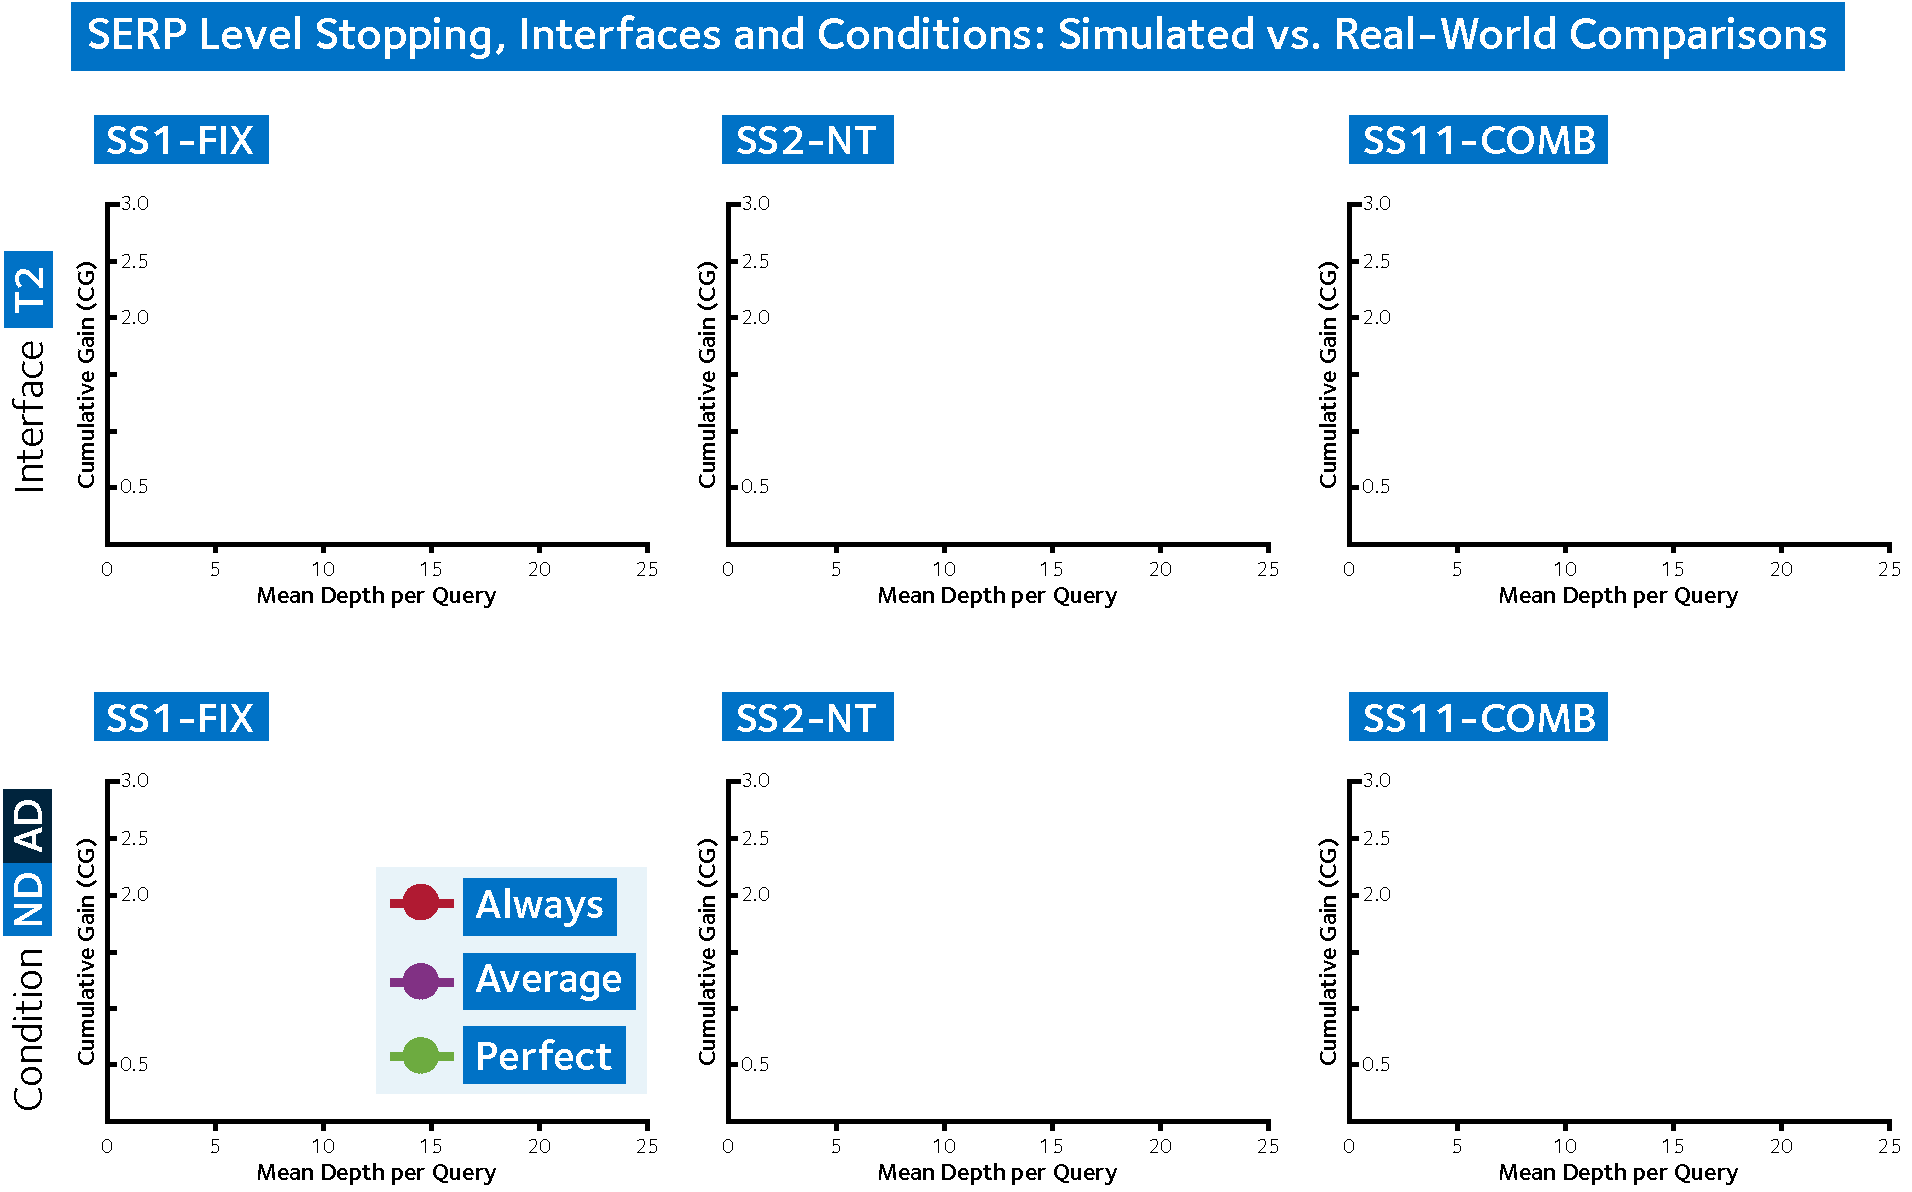
\includegraphics{figures/ch9-comparison_plots.pdf}}
    \caption[Real-world comparisons over the~\gls{acr:serp} decision point]{Plots reporting the comparison runs, reporting the MSE vs. the mean depth per query. Runs over interface \blueboxbold{T2} (top) and condition \dualbluebox{ND}{AD} (bottom) are shown, for the three trialled result summary level stopping strategies.~\gls{acr:serp} level decision point implementations are also shown. Also included are dashed lines denoting the mean depth per query reached by the real-world subjects of the corresponding user study. Note that the mean depth per query is limited from \emph{5} to \emph{20} to highlight what happens around the mean real-world click depths.}
    \label{fig:ch9_comparison_plots}
\end{figure}

Figure~\ref{fig:ch9_comparison_plots} presents six plots, one for each of the three result summary level stopping strategies: \blueboxbold{SS1-FIX}; \blueboxbold{SS2-NT}; and \blueboxbold{SS5-COMB}. These are duplicated over interface \blueboxbold{T2} and condition \dualbluebox{ND}{AD}. Each of the plots illustrates the mean depth per query to which searchers traversed result lists to (represented along the $x$ axis). This is plotted against the MSE\footnote{Refer to Section~\ref{sec:method:simulation:runs:comparison} on page~\pageref{sec:method:simulation:runs:comparison} for further information on how we computed the \emph{Mean Squared Error (MSE)} for our comparisons.} of the real-world vs. simulated searcher click depths (thus considering stopping behaviours). Each point on the plotted lines represents how close the click depth approximation was on average for a given stopping threshold parameter configuration. The closer the MSE value tends towards zero, the closer the simulated searcher's approximation to actual stopping behaviours. Each plot also presents one of the three trialled~\gls{acr:serp} level stopping decision points, from \dualbluebox{SERP}{Always}, \dualbluebox{SERP}{Average}, and \dualbluebox{SERP}{Perfect}. The plots demonstrate how approximations from each of the implementations differ across interfaces/conditions and result summary level stopping strategies. We also include the mean real-world click depths for a straightforward visual comparison, represented as vertical dashed lines. These differ between interface \blueboxbold{T2} and \dualbluebox{ND}{AD}, as shown in Figures~\ref{fig:ch7_sim_comparison_plots} (page~\pageref{fig:ch7_sim_comparison_plots}) and~\ref{fig:ch8_sim_comparison_plots} (page~\pageref{fig:ch8_sim_comparison_plots}), respectively. Note also truncated \emph{x} and \emph{y} axes. As all plotted lines were close together, we altered the axes to better highlight the approximations when the MSE values were at their lowest.

\begin{table}[t!]
    \caption[Lowest MSE values for~\gls{acr:serp} decision point implementations]{Results from the simulated comparison runs, showing the \emph{lowest} \genericblack{MSE} value reached over each of the three result summary level stopping strategies trialled. These are reported over the \dualbluebox{SERP}{Always} \emph{(baseline),} \dualbluebox{SERP}{Average} and \dualbluebox{SERP}{Perfect}~\gls{acr:serp} level stopping decision point implementations. The stopping strategy yielding the lowest MSE for both \blueboxbold{T2} and \dualbluebox{ND}{AD} are \darkbluebox{highlighted}. Note that for combination strategy \blueboxbold{SS5-COMB}, \emph{x\textsubscript{2},x\textsubscript{4}} are shown as \genericblack{x\textsubscript{n}} column.}
    \label{tbl:ch9_comparisons_table}
    \renewcommand{\arraystretch}{1.8}
    \begin{center}
        \begin{tabulary}{\textwidth}{L{0.25cm}@{\CS}L{3.55cm}@{\CS}D{1.4cm}@{\CS}D{1.4cm}@{\CSONEHALF}D{1.4cm}@{\CS}D{1.4cm}@{\CSONEHALF}D{1.4cm}@{\CS}D{1.4cm}@{\CS}}
            
            & & \multicolumn{2}{@{\hskip 0pt}c@{\CSONEHALF}}{\dbluecell\small\textbf{Always}} & \multicolumn{2}{@{\hskip 0pt}c@{\CSONEHALF}}{\dbluecell\small\textbf{Average}} & \multicolumn{2}{@{\hskip 0pt}c@{\hskip 16pt}}{\dbluecell\small\textbf{Perfect}}\\
            
            \RS & & \lbluecell\small\textbf{x\textsubscript{n}} & \lbluecell\small\textbf{MSE} & \lbluecell\small\textbf{x\textsubscript{n}} & \lbluecell\small\textbf{MSE} & \lbluecell\small\textbf{x\textsubscript{n}} & \lbluecell\small\textbf{MSE} \\
            
            % T2
            \RS \multirow{3}{*}{\hspace*{-2mm}\rotatebox{90}{\hspace*{-7mm}\footnotesize Int. \blueboxbold{\textbf{T2}}}} & \lbluecell\small\textbf{SS1-FIX} & \cell \small \hspace*{-1mm} 21 & \cell \small \hspace*{-1mm} 74.04 & \cell \hspace*{-1mm} \small 24 & \dbluecell \small \hspace*{-1mm} 70.68 & \cell \small \hspace*{-1mm} 24 & \cell \hspace*{-1mm} \small 76.94 \\
            \RS  & \lbluecell\small\textbf{SS2-NT} & \cell \small \hspace*{-1mm} 15 & \cell \small \hspace*{-1mm} 77.76 & \cell \hspace*{-1mm} \small 21 & \dbluecell \small \hspace*{-1mm} 72.12 & \cell \small \hspace*{-1mm} 18 & \cell \hspace*{-1mm} \small 82.06 \\
            
            \RS  & \lbluecell\small\textbf{SS5-COMB} & \cell \small \hspace*{-1mm} 21,6 & \cell \small \hspace*{-1mm} 72.81 & \cell \hspace*{-1mm} \small 21,10 & \dbluecell \small \hspace*{-1mm} 70.23 & \cell \small \hspace*{-1mm} 21,7 & \cell \hspace*{-1mm} \small 77.89 \\
            
            % ND-AD
            \RS\RS\RS \multirow{3}{*}{\hspace*{-2mm}\rotatebox{90}{\hspace*{-7mm}\footnotesize Cdn. \textbf{\dualbluebox{ND}{AD}}}} & \lbluecell\small\textbf{SS1-FIX} & \cell \small \hspace*{-1mm} 21 & \cell \small \hspace*{-1mm} 168.39 & \cell \hspace*{-1mm} \small 24 & \cell \small \hspace*{-1mm} 176.98 & \cell \small \hspace*{-1mm} 24 & \dbluecell \hspace*{-1mm} \small 164.97 \\
            \RS  & \lbluecell\small\textbf{SS2-NT} & \cell \small \hspace*{-1mm} 18 & \cell \small \hspace*{-1mm} 175.39 & \cell \hspace*{-1mm} \small 24 & \dbluecell \small \hspace*{-1mm} 169.52 & \cell \small \hspace*{-1mm} 21 & \cell \hspace*{-1mm} \small 169.85 \\
            \RS  & \lbluecell\small\textbf{SS5-COMB} & \cell \small \hspace*{-1mm} 21,5 & \cell \small \hspace*{-1mm} 162.81 & \cell \hspace*{-1mm} \small 24,8 & \cell \small \hspace*{-1mm} 168.26 & \cell \small \hspace*{-1mm} 21,5 & \dbluecell \hspace*{-1mm} \small 160.69 \\

        \end{tabulary}
        \end{center}
    \end{table}

At a glance, the small difference between MSE values demonstrates that there is not much of a difference between the three~\gls{acr:serp} level stopping decision point implementations. To aid in the reporting of our results, we also include a table of MSE values. Table~\ref{tbl:ch9_comparisons_table} reports the lowest MSE values that were attained across each of the~\gls{acr:serp} level stopping decision point implementations and stopping strategies, over \blueboxbold{T2} and \dualbluebox{ND}{AD}. Along with the MSE values are the stopping parameter threshold(s) that were used to attain the lowest MSE for each combination. For combination stopping strategy \blueboxbold{SS5-COMB}, we once again report $x_2$ and $x_4$ for the thresholds, in that order. We also \darkbluebox{highlight} in the table the lowest MSE values over the three~\gls{acr:serp} level stopping decision point implementations, considering each result summary level stopping strategy in turn.

From Table~\ref{tbl:ch9_comparisons_table}, we note that over interface \blueboxbold{T2}, the \dualbluebox{SERP}{Average}~\gls{acr:serp} level stopping decision point consistently yielded the lowest MSE values over the three result summary level stopping strategies trialled. This is closely followed by our baseline approach, \dualbluebox{SERP}{Always}, with \dualbluebox{SERP}{Perfect} consistently offering the poorest approximations of mean real-world searcher approximations. This result is intuitive -- real-world searchers would have been unlikely to correctly judge the scent of a~\gls{acr:serp} with 100\% accuracy, and thus would mean that the upper bound \dualbluebox{SERP}{Perfect} implementation would be furthest from mean real-world stopping behaviours. In contrast, a stochastic approach offered by \dualbluebox{SERP}{Average} would intuitively yield better approximations. Although real-world searchers would not have rolled a die to determine whether a~\gls{acr:serp} is worth examining, they would have had the flexibility to abandon~\glsplural{acr:serp} that they felt did not offer a good scent. This flexibility is provided to the \dualbluebox{SERP}{Average} simulated searcher. An interesting observation for interface \blueboxbold{T2} is the higher stopping parameter threshold(s) that were found to offer the lowest MSE values. This demonstrates that the mean real-world searcher stopping behaviours over this interface is that of a tolerant searcher, who is willing to examine results to greater depths on average, before deciding to stop.

The trends that we observe for interface \blueboxbold{T2} in Table~\ref{tbl:ch9_comparisons_table} can also be demonstrated by close examination of the corresponding (top) plots in Figure~\ref{fig:ch9_comparison_plots}. Close examination shows that across varying mean depths per query, the general trends observed from Table~\ref{tbl:ch9_comparisons_table} hold -- \dualbluebox{SERP}{Perfect} and \dualbluebox{SERP}{Always} consistently offered poorer approximations than \dualbluebox{SERP}{Average}, which consistently offered the lowest MSE values.

Results over interface \dualbluebox{ND}{AD} are different from those of interface \blueboxbold{T2}. Examining Table~\ref{tbl:ch9_comparisons_table}, we observe that \dualbluebox{SERP}{Average} yielded the best mean searcher stopping approximation for \dualbluebox{SS2-NT}{@24}. Interestingly however, we find that the lowest MSE values for \dualbluebox{SS1-FIX}{@24} and \dualbluebox{SS5-COMB}{@21,5} were yielded by the \dualbluebox{SERP}{Perfect}~\gls{acr:serp} level stopping decision point implementation. This perhaps demonstrates that the change in task goals (from time-limited for \blueboxbold{T2} to find $x$ for \dualbluebox{ND}{AD}) influences the~\gls{acr:serp} level decision making of real-world searchers on average. Results show that under \blueboxbold{SS1-FIX} and \blueboxbold{SS5-COMB}, searchers under \dualbluebox{ND}{AD} were better able to discern between poor and high quality~\glsplural{acr:serp}. We provide a discussion into this result in Section~\ref{sec:conclusions:discussion}.

\begin{table}[t!]
    \caption[Additional results for comparison runs]{Additional results from the searcher comparison runs, reporting the mean depth per query (\genericblack{DQ}), the mean level of \genericblack{CG}, and mean interactive precision (\genericblack{iP}). These values were attained using the configurations yielding the lowest MSE (refer to Table~\ref{tbl:ch9_comparisons_table}), indicating the best approximation to real-world stopping behaviours. We also include the mean real-world searcher values (\genericblack{RW}) over \blueboxbold{T2} and \dualbluebox{ND}{AD} for a direct comparison.}
    \label{tbl:ch8_additional_comparisons_table}
    \renewcommand{\arraystretch}{1.8}
    \begin{center}
        \begin{tabulary}{\textwidth}{L{0.25cm}@{\CS}L{2.18cm}@{\CS}D{0.895cm}@{\CS}D{0.895cm}@{\CS}D{0.895cm}@{\CSONEHALF}D{0.895cm}@{\CS}D{0.895cm}@{\CS}D{0.895cm}@{\CSONEHALF}D{0.895cm}@{\CS}D{0.895cm}@{\CS}D{0.895cm}@{\CSONEHALF}}
            
            & & \multicolumn{3}{@{\hskip 0pt}c@{\CSONEHALF}}{\dbluecell\small\textbf{Always}} & \multicolumn{3}{@{\hskip 0pt}c@{\CSONEHALF}}{\dbluecell\small\textbf{Average}} & \multicolumn{3}{@{\hskip 0pt}c@{\CSONEHALF}}{\dbluecell\small\textbf{Perfect}}\\
            
            \RS & & \lbluecell\small\textbf{DQ} & \lbluecell\small\textbf{CG} & \lbluecell\small\textbf{iP} & \lbluecell\small\textbf{DQ} & \lbluecell\small\textbf{CG} & \lbluecell\small\textbf{iP} & \lbluecell\small\textbf{DQ} & \lbluecell\small\textbf{CG} & \lbluecell\small\textbf{iP} \\
            
            % T2
            
            \RS \multirow{4}{*}{\hspace*{-2mm}\rotatebox{90}{\hspace*{-5mm}\footnotesize Interface \blueboxbold{\textbf{T2}}}} & \dbluecell\small\textbf{RW} & \cell \small \hspace*{-1mm} 14.39 & \cell \small \hspace*{-1mm} 2.36 & \cell \hspace*{-1mm} \small 2.47 & \cell \small \hspace*{-1mm} 14.39 & \cell \small \hspace*{-1mm} 2.36 & \cell \hspace*{-1mm} \small 2.47 & \cell \small \hspace*{-1mm} 14.39 & \cell \small \hspace*{-1mm} 2.36 & \cell \hspace*{-1mm} \small 2.47 \\
            \RS & \lbluecell\small\textbf{SS1-FIX} & \cell \small \hspace*{-1mm} 14.67 & \cell \small \hspace*{-1mm} 2.14 & \cell \hspace*{-1mm} \small 1.41 & \dbluecell \small \hspace*{-1mm} 12.35 & \dbluecell \small \hspace*{-1mm} 1.82 & \dbluecell \hspace*{-1mm} \small 1.17 & \cell \small \hspace*{-1mm} 13.68 & \cell \small \hspace*{-1mm} 2.16 & \cell \hspace*{-1mm} \small 1.41 \\
            \RS  & \lbluecell\small\textbf{SS2-NT} & \cell \small \hspace*{-1mm} 13.81 & \cell \small \hspace*{-1mm} 2.15 & \cell \hspace*{-1mm} \small 1.42 & \dbluecell \small \hspace*{-1mm} 13.70 & \dbluecell \small \hspace*{-1mm} 1.98 & \dbluecell \hspace*{-1mm} \small 1.27 & \cell \small \hspace*{-1mm} 13.06 & \cell \small \hspace*{-1mm} 2.22 & \cell \hspace*{-1mm} \small 1.45 \\
            \RS  & \lbluecell\small\textbf{SS5-COMB} & \cell \small \hspace*{-1mm} 15.22 & \cell \small \hspace*{-1mm} 2.08 & \cell \hspace*{-1mm} \small 1.34 & \dbluecell \small \hspace*{-1mm} 13.35 & \dbluecell \small \hspace*{-1mm} 1.93 & \dbluecell \hspace*{-1mm} \small 1.25 & \cell \small \hspace*{-1mm} 13.11 & \cell \small \hspace*{-1mm} 1.99 & \cell \hspace*{-1mm} \small 1.30 \\
            
            % ND-AD
            \RS\RS\RS \multirow{4}{*}{\hspace*{-2mm}\rotatebox{90}{\hspace*{-7mm}\footnotesize Condition \textbf{\dualbluebox{ND}{AD}}}} & \dbluecell\small\textbf{RW} & \cell \small \hspace*{-1mm} 13.94 & \cell \small \hspace*{-1mm} 3.49 & \cell \hspace*{-1mm} \small 2.22 & \cell \small \hspace*{-1mm} 13.94 & \cell \small \hspace*{-1mm} 3.49 & \cell \hspace*{-1mm} \small 2.22 & \cell \small \hspace*{-1mm} 13.94 & \cell \small \hspace*{-1mm} 3.49 & \cell \hspace*{-1mm} \small 2.22 \\
            \RS & \lbluecell\small\textbf{SS1-FIX} & \cell \small \hspace*{-1mm} 12.89 & \cell \small \hspace*{-1mm} 2.55 & \cell \hspace*{-1mm} \small 1.66 & \cell \small \hspace*{-1mm} 9.61 & \cell \small \hspace*{-1mm} 1.84 & \cell \hspace*{-1mm} \small 1.20 & \dbluecell \small \hspace*{-1mm} 13.06 & \dbluecell \small \hspace*{-1mm} 2.59 & \dbluecell \hspace*{-1mm} \small 1.69 \\
            \RS  & \lbluecell\small\textbf{SS2-NT} & \cell \small \hspace*{-1mm} 13.34 & \cell \small \hspace*{-1mm} 2.73 & \cell \hspace*{-1mm} \small 1.77 & \dbluecell \small \hspace*{-1mm} 11.33 & \dbluecell \small \hspace*{-1mm} 2.12 & \dbluecell \hspace*{-1mm} \small 1.38 & \cell \small \hspace*{-1mm} 13.35 & \cell \small \hspace*{-1mm} 2.78 & \cell \hspace*{-1mm} \small 1.84 \\
            \RS  & \lbluecell\small\textbf{SS5-COMB} & \cell \small \hspace*{-1mm} 14.16 & \cell \small \hspace*{-1mm} 2.69 & \cell \hspace*{-1mm} \small 1.75 & \cell \small \hspace*{-1mm} 11.14 & \cell \small \hspace*{-1mm} 2.05 & \cell \hspace*{-1mm} \small 1.34 & \dbluecell \small \hspace*{-1mm} 11.94 & \dbluecell \small \hspace*{-1mm} 2.53 & \dbluecell \hspace*{-1mm} \small 1.66 \\

        \end{tabulary}
        \end{center}
        \vspace*{-5mm}
    \end{table}

Table~\ref{tbl:ch8_additional_comparisons_table} also provides additional information on the comparison runs. The table reports the mean depth per query (\genericblack{DQ}), \genericblack{CG} and interactive precision (\genericblack{iP}) attained across each of the~\gls{acr:serp} level stopping decision point implementations and result summary level stopping strategies, again over interface \blueboxbold{T2} and condition \dualbluebox{ND}{AD}. To allow for easy comparison, we also include the real-world mean depth per query,~\gls{acr:cg} and interactive precision values (row \genericblack{RW}) across the interface and condition examined.

Trends from Table~\ref{tbl:ch8_additional_comparisons_table} show that as we tend from \dualbluebox{SERP}{Always} to \dualbluebox{SERP}{Average}, we generally observed a \emph{drop} in the~\gls{acr:cg} attained by the simulated searchers. Over interface \blueboxbold{T2} for example,~\gls{acr:cg} for \dualbluebox{SS2-NT}{@15} dropped from $2.15$ for \dualbluebox{SERP}{Always} to $1.98$ for \dualbluebox{SS2-NT}{@21} for \dualbluebox{SERP}{Average}. Unsurprisingly, we observed that under \dualbluebox{SERP}{Perfect},~\gls{acr:cg} was generally higher than the other two~\gls{acr:serp} level stopping decision point implementations. Corresponding interactive precision rose and fell with the~\gls{acr:cg} attained -- an intuitive result. As a reminder, results in Table~\ref{tbl:ch8_additional_comparisons_table} demonstrate the levels of~\gls{acr:cg} and interactive precision attained using the configurations that yielded the lowest MSE values. These were computed with respect to click depths. As such, these values do not correspond to the maximum level of performance that could be attained; rather, they demonstrate the best performance that would have been attained by a searcher had a given result summary level stopping strategy been rigidly followed. From the \genericblack{RW} values for interface \blueboxbold{T2} and \dualbluebox{ND}{AD}, we see that the simulated searcher~\gls{acr:cg} and interactive precision values fall below the real-world equivalents.

To conclude our analysis of the comparison runs, we performed a series of statistical tests to demonstrate if significant differences in terms of approximations existed. Like our \emph{what-if} performance runs described in Section~\ref{sec:serp:results:comparisons} above, we considered the best-performing~\gls{acr:serp} level stopping decision point implementation and result summary level stopping strategy combination, comparing the MSE values attained there against the other two~\gls{acr:serp} level decision point implementations. Given the closeness of each of the~\gls{acr:serp} level decision point implementations, no significant differences were found over any combination of result summary level stopping strategy, or interface/condition. Therefore, results show that there is supporting evidence for \darkblueboxbold{SERP-RQ2}, albeit not statistically significant. Interesting findings between interface \blueboxbold{T2} and \dualbluebox{ND}{AD} will receive further discussion in Section~\ref{sec:conclusions:discussion}.

\section{Chapter Summary}
In this chapter, we conducted a series of simulations that empirically tested the~\gls{acr:csm}, complete with the new~\gls{acr:serp} level stopping decision point (as discussed in Section~\ref{sec:csm:advancements:stopping} on page~\pageref{sec:csm:advancements:stopping}). We observed improvements in:

\begin{itemize}
    \item{\darkblueboxbold{SERP-RQ1} overall performance; and}
    \item{\darkblueboxbold{SERP-RQ2} approximations to actual real-world searcher stopping behaviours.}
\end{itemize}

Results were significantly improved in terms of overall~\gls{acr:cg} attained between the upper-bound \dualbluebox{SERP}{Perfect} implementation (only examine a~\gls{acr:serp} if it appears to yield a high scent), and the baseline \dualbluebox{SERP}{Always} implementation (always examine a~\gls{acr:serp}, regardless of perceived quality). Improvements were consistent across our trialled interface and condition, as well as across different result summary level stopping strategies. Our stochastic implementation, \dualbluebox{SERP}{Always}, consistently ranked between our baseline and upper-bound implementation.

Results pertaining to \darkblueboxbold{SERP-RQ2} were however not significant, with our findings differing across interface \blueboxbold{T2} and condition \dualbluebox{ND}{AD}. Over interface \blueboxbold{T2}, we found that the \dualbluebox{SERP}{Average} implementation consistently yielded the better approximations over \dualbluebox{SERP}{Perfect} and \dualbluebox{SERP}{Always} -- an intuitive result. Differences, as previously mentioned, were however very slight and not statistically significant -- MSE approximations varied in the region of ten units. Over condition \dualbluebox{ND}{AD}, we found that \dualbluebox{SERP}{Average} and \dualbluebox{SERP}{Perfect} offered the best approximations -- an interesting result. This suggests that when task goals vary, a searcher's behaviour with respect obtaining an initial impression of a~\gls{acr:serp} also varies.

Overall, we find that including the new~\gls{acr:serp} level stopping decision point ultimately leads to better performing and more realistic simulations of interaction.

%We now turn our attention to the final chapter, which provides a discussion on the findings from this -- and other prior contributory chapters -- before concluding the work that this thesis has presented.

\newpage
\thispagestyle{empty}
\mbox{}